\documentclass[dutch]{style/tudelft-report}

\usepackage{acronym}
\usepackage{wrapfig}
\acrodef{sig}[SIG]{Software Improvement Group}
\acrodef{rx}[Rx]{Reactive Extensions}
\acrodef{tfs}[TFS]{Team Foundation Server}
\acrodef{mvp}[MVP]{Minimum Viable Product}
\acrodef{paas}[PaaS]{Platform as a Service}
\acrodef{KNSB}[KNSB]{Koninklijke Nederlandsche Schaatsenrijders Bond}
\acrodef{pcl}[PCL]{Portable Class Library}
%\acrodef{label}[acronym]{written out form}
\usepackage{longtable}
\usepackage{array}

\begin{document}

%% Use Roman numerals for the page numbers of the title pages and table of
%% contents.

\frontmatter

\title[Bachelorproject \\ ~ \\ Orientatieverslag]{Vantage Practice}
\author{H.J.\ Banken \\ P.A.\ van Hesteren \\ H.T.D.\ Visser}
\affiliation{Technische Universiteit Delft}

\begin{titlepage}

\begin{center}

%% Insert the TU Delft logo at the bottom of the page.
\begin{tikzpicture}[remember picture,overlay]
    \node at (current page.south)[anchor=south,inner sep=0pt]{
        
\includegraphics{style/cover/logo}
    };
\end{tikzpicture}

\begin{tikzpicture}[remember picture,overlay]
    \node at (current page.south)[anchor=south,inner sep=80pt]{
        
\includegraphics[scale=0.7]{style/cover/emando}
    };
\end{tikzpicture}

%% Extra whitespace at the top.
\vspace*{2\bigskipamount}

%% Print the title in cyan.
{\makeatletter
\titlestyle\color{tudelft-cyan}\Huge\@title
\makeatother}

\bigskip
\bigskip

{\makeatletter
\titlestyle\color{tudelft-cyan}\LARGE Trainingsapp voor Baansporten
\makeatother}

%% Print the optional subtitle in black.
{\makeatletter
\ifx\@subtitle\undefined\else
    \bigskip
    \titlefont\titleshape\Large\@subtitle
\fi
\makeatother}

\bigskip
\bigskip

%by
door

\bigskip
\bigskip

%% Print the name of the author.
{\makeatletter
\titlefont\Large\bfseries Herman Banken
\makeatother}

\bigskip

{\makeatletter
\titlefont\Large\bfseries Patrick van Hesteren
\makeatother}

\bigskip

{\makeatletter
\titlefont\Large\bfseries Hylke Visser
\makeatother}

\vfill

\begin{tabular}{lll}
%% Add additional information here, per faculty requirements, e.g
%    Student number: & 1234567 \\
%    Project duration: & \multicolumn{2}{l}{March 1, 2012 -- January 1, 2013} \\
    TU Coach: & Dr.ir. C.\ Bezemer \\
    Projectbegeleider: & J.\ Stokking
\end{tabular}

%% Only include the following lines if confidentiality is applicable.
\bigskip
\bigskip
%\emph{This thesis is confidential and cannot be made public until December 31, 2013.}
%\emph{Op dit verslag is geheimhouding van toepassing tot en met 31 december 2013.}

\bigskip
\bigskip

\bigskip
\bigskip
%An electronic version of this thesis is available at \url{http://repository.tudelft.nl/}.
%Een elektronische versie van dit verslag is beschikbaar op \url{http://repository.tudelft.nl/}.

\end{center}

\end{titlepage}

\chapter{Voorwoord}
Dit document is het oriëntatieverslag, dat is geschreven voor aanvang van het bachelor-project “Trainingsapp voor Baansporten”. 

\bigskip

\noindent
Dit project wordt door Herman Banken, Patrick van Hesteren en Hylke Visser uitgevoerd als Bachelor Eindproject voor de Bachelor Technische Informatica aan de Technische Universiteit Delft. Het project wordt uitgevoerd tussen 22 april en 27 juni 2014. Het project wordt uitgevoerd bij het bedrijf \textbf{Emando} onder begeleiding van Johan Stokking en wordt vanuit de Technische Universiteit Delft begeleid door Cor-Paul Bezemer.

\bigskip

\begin{flushright}
{\makeatletter\itshape
    Herman Banken \\
    Patrick van Hesteren \\
    Hylke Visser \\
    Delft, April 2014
\makeatother}
\end{flushright}

\tableofcontents

%% Use Arabic numerals for the page numbers of the chapters.
\mainmatter

\chapter{Ori\"entatieverslag} \label{ch:orientatie} \section{Introductie}

Aan de hand van de projectopdracht, ons Plan van Aanpak en gesprekken met Johan en Cor-Paul hebben we dit Orientatieverslag opgesteld. Dit verslag zal worden gebruikt om inzicht te verkrijgen in de mogelijke technieken voor het ontwikkelen van mobiele applicaties en server back-ends, geschikt voor onze toepassing. Tevens zullen we hier onze keuzes voor bepaalde technieken motiveren.

\section{Abcdefg}
\label{sec:alphabet}


%% Use letters for the chapter numbers of the appendices.
\appendix

\addtocontents{toc}{\protect\setcounter{tocdepth}{1}}

\chapter{Plan van Aanpak} \label{ch:plan-van-aanpak} \section{Introductie}

\ifx\aanleiding\undefined
\newcommand{\aanleiding}{}

\begin{wrapfigure}{r}{4cm}
  \begin{center}
    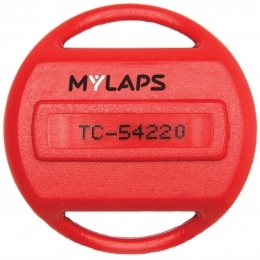
\includegraphics[width=4cm]{style/images/transponder}
  \end{center}
  \caption{MyLaps ProFlex transponder, op schaal}
  \label{fig:transponder}
  \vspace{15mm}
\end{wrapfigure}

In baansporten is de laatste jaren een ontwikkeling gaande om tijdregistratie te digitaliseren door het gebruik van transponders (bijvoorbeeld de MyLaps ProFlex transponder in Figuur~\ref{fig:transponder}) en detectie-lussen (Figuur~\ref{fig:detection-loop}) in de baan. Door deze ontwikkeling zijn nieuwe mogelijkheden ontstaan om ook naast het wedstrijdmoment de sportprestaties in te zien. Het constateren van de hierna genoemde nieuwe mogelijkheden was de aanleiding van dit project.

\begin{wrapfigure}{r}{4cm}
  \begin{center}
    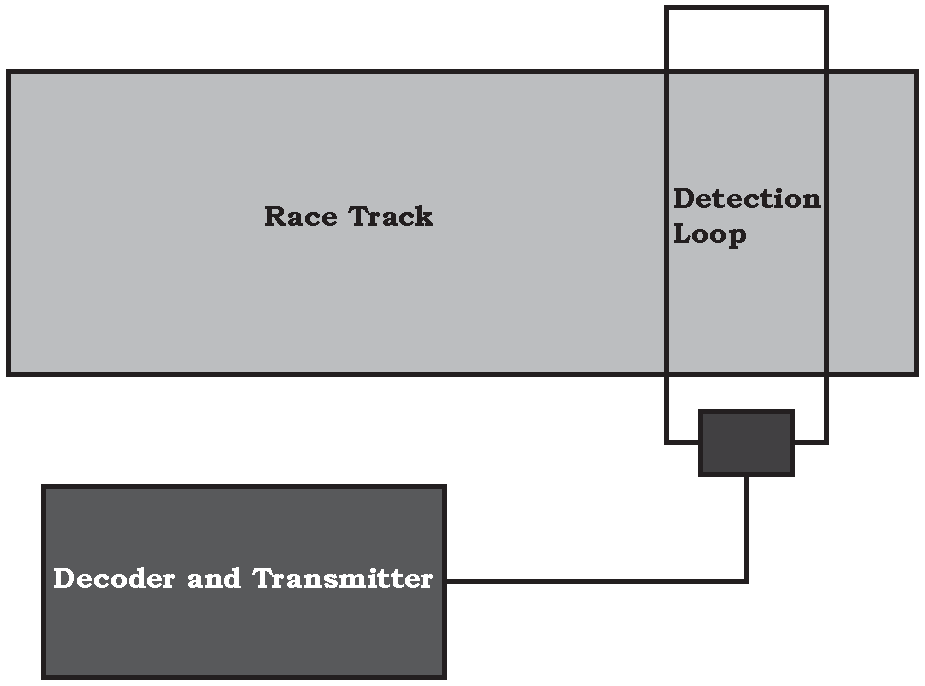
\includegraphics[width=4cm]{style/images/DetectionLoop}
  \end{center}
  \caption{Een schema van een detectielus en en decoder}
  \label{fig:detection-loop}
  \vspace{5mm}
\end{wrapfigure}

Een grote speler op de tijdregistratie-markt is MyLaps\footnote{\url{http://www.mylaps.com}}. Dit bedrijf installeert en beheert detectie-lussen en is actief bij diverse sporten zoals schaatsen, wielrennen, zwemmen, atletiek en diverse motorsporten. Bij sporten met permanente banen liggen de detectie-lussen het gehele jaar in de baan. Er bestaat de mogelijkheid om op de website van MyLaps doorkomst-tijden in te zien. De informatie die uit deze tijden is af te leiden, wordt door sporters als erg waardevol gezien om zich willen blijven verbeteren, waardoor er steeds meer getraind wordt met deze transponders.

\begin{figure}
  \begin{center}
    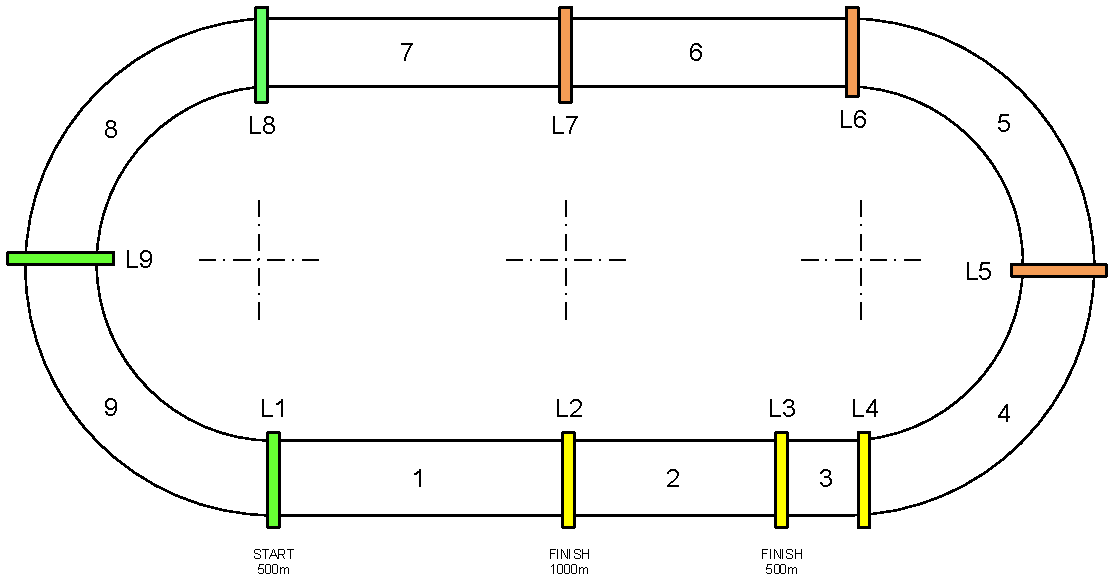
\includegraphics[width=0.8\textwidth]{style/images/BaanoverzichtHaarlem}
  \end{center}
  \caption{L1 tot en met L9 zijn de negen MyLaps transponderlussen in Haarlem}
  \label{fig:track-transponders}
\end{figure}

Voor aanvang van het seizoen worden door MyLaps detectielussen geïnstalleerd. De lussen bevinden zich in het ijs of onder het houten oppervlak van een baanwielrenbaan. Elke lus heeft een elektromagnetisch veld. Wanneer een sporter met transponder over dat veld heen rijdt, wordt de transponder geactiveerd en stuurt deze een unieke puls, die de lus opvangt. De MyLaps X2 server die aan de lussen zit aangesloten stuurt vervolgens het signaal door naar de MyLaps Cloud.

Het huidige gebruik van transponders - buiten wedstrijden - is voornamelijk achteraf, terwijl juist tijdens de training zowel sporter als coach het meeste bezig zijn met de prestaties. Het is daarom wenselijk om de resultaten in real-time door te geven aan coaches en sporters zelf.

Op veel banen zijn meerdere detectie-lussen geïnstalleerd, terwijl er op de website van MyLaps slechts één wordt ontsloten. In Thialf, de schaatsbaan in Heerenveen, Friesland, liggen bijvoorbeeld twaalf detectie-lussen, in Haarlem (Figuur~\ref{fig:track-transponders}) negen en op de andere schaatsbanen liggen er tenminste twee. Door de data van meerdere lussen te combineren is een betere indicatie te maken van de snelheid van sporters.

\begin{wrapfigure}{r}{0.4\textwidth}
 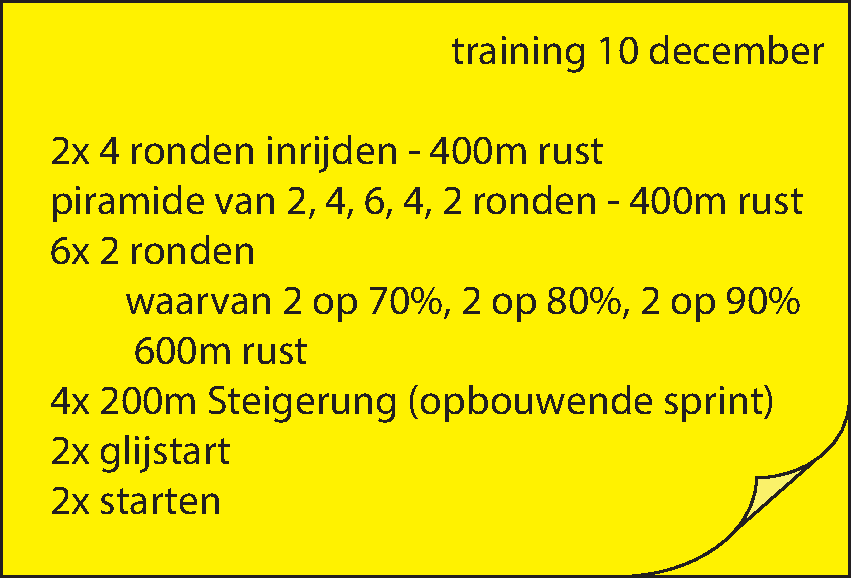
\includegraphics[width=0.4\textwidth]{style/images/training}
 \caption{Een typisch schaats-trainingsschema}
\end{wrapfigure}

Trainingen, bij bijvoorbeeld schaatsen, bestaan uit losse trainingsonderdelen. Allround schaatsers moeten bijvoorbeeld 4 ronden warmrijden, dan 6 keer 2 ronden sprinten, dan 4 keer een sprintje van 200 meter, 2 keer een glijstart en dan 2 keer een echte start bij de coach, vanuit de zijkant van de baan. Tussendoor is er rust, zo is het gebruikelijk om na een opdracht tenminste 400 meter uit te glijden. Het verschil tussen training en rust is af te leiden uit de verhouding tot de maximale snelheid.

Veel trainingselementen bestaan dus uit korte opdrachten, waar het juist om snelheid gaat. Een enkele lus is dan niet afdoende, omdat de rust voor of na de opdracht mee wordt gewogen. Sporters starten en stoppen namelijk niet precies boven de lus, maar starten vaak na de bocht en stoppen afhankelijk van de afstand van de opdracht op een willekeurig punt. 

Andere trainingen van bijvoorbeeld lange afstands- of marathonschaatsers kunnen bestaan uit één element: de hele training lang schaatsen, zonder overeind te komen. Wanneer er op tactische punten detectie-lussen geïnstalleerd zijn, is er bijvoorbeeld ook onderscheid te maken tussen bochten en de rechte stukken. Bij sporten met een ronde baan verschilt de snelheid in de bocht namelijk erg met die op het rechte eind. Deze vergelijking gebeurt nu al in Thialf, in het professionele circuit tijdens wedstrijden op televisie.

Topsporters zijn enorm prestatiegericht en als je al aan de top zit, dan kunnen kleine aanpassingen aan je techniek, ademhaling et cetera, grote verschillen maken. Coaches van professionele teams houden zich daarom bezig met allerhande analyses. Naast ademanalyse en hartslag monitoring, is het in Thialf bijvoorbeeld ook mogelijk om (van maximaal 20 schaatsers) continu de positie te bepalen met een in-door positioning system (IPS) ontwikkeld door InnoSportLab\footnote{\url{http://www.innosportlabthialf.nl}}.

Al deze geavanceerde analyses zijn echter te duur en kosten te veel tijd voor recreatieve sporters. MyLaps X2 biedt in combinatie met ons eindproduct recreatieve sporters toch een manier om analyses uit te voeren en zich naar een hoger niveau te tillen.
\fi

Aan de hand van de projectopdracht, te lezen in Sectie~\ref{sec:projectopdracht}, en gesprekken met Johan en Cor-Paul hebben we dit Plan van Aanpak opgesteld. Dit Plan van Aanpak zal worden gebruikt als houvast bij het uitvoeren van het project en wordt daarom ook goedgekeurd door alle betrokken partijen.

In dit document zal eerst de projectopdracht aan bod komen en zal worden toegelicht hoe deze tot stand is gekomen. Vervolgens wordt toegelicht op welke wijze we te werk zullen gaan en wat onze tijdsplanning is. Hierna wordt iets dieper ingegaan op de procesmatige inrichting van het project. Tot slot zal er nog aandacht worden besteed aan kwaliteitsborging.

\section{Projectopdracht}
\label{sec:projectopdracht}
\subsection{Opdrachtomgeving}

Emando is een bedrijf dat zich momenteel onder andere richt op het ontwikkelen van Vantage. Een onderdeel van Vantage is een systeem voor tijdregistratie tijdens wedstrijden in baansporten. Een groot deel van de door Vantage gebruikte infrastructuur zou ook gebruikt kunnen worden voor de recreatieve- of amateurvariant van de sport. Hiervoor zou het project ``Trainingsapp voor Baansporten'' verschillende mogelijkheden moeten bieden.

\subsection{Doelstelling project}
Het project is bedoeld als pilot. Dit houdt in dat het een mogelijke toevoeging zou kunnen zijn aan het bestaande Vantage platform, dat momenteel vooral gericht is op wedstrijden. Emando kan met dit project ook een dienst aanbieden voor recreatieve sporters en voor trainingen om hun prestaties in te zien en te vergelijken.

\subsection{Opdrachtformulering}
In overleg met Emando is de projectopdract als volgt gedefinieerd:

\begin{quotation}
\itshape
Het ontwerpen en ontwikkelen van een systeem voor het weergeven en analyseren van (live) recreatieve en trainingsdata in de context van baansporten (bijvoorbeeld schaatsen en baanwielrennen). Dit systeem zal realtime gegevens van de baan, maar ook opgeslagen gegevens uit het verleden, inzichtelijk maken voor sporters, coaches en eventuele toeschouwers (volgers). Daarnaast zal er de mogelijkheid zijn om een sociale component en een competitie element toe te voegen, en een mogelijkheid om aggregatie op data uit te voeren.

Het systeem ondersteunt het sporten: sporters hoeven hun training niet te onderbreken, doordat audio-cue's en sport-specifieke schermen geïmplementeerd worden. De sociale component bestaat uit het volgen van vrienden (mede-sporters) en het delen van resultaten. Het competitie element zal een virtuele competitie tussen vrienden omvatten.

Technisch gezien zal er een scheiding gemaakt worden tussen de diverse toepassingen (clients) en de API. De API biedt toegang tot realtime data en de diverse modulaire (sport-specifieke) aggregaties, waarbij de mogelijkheid bestaat voor bijvoorbeeld coaches om te abonneren op meerdere sporters. De API zal gekoppeld worden op bestaande systemen die data van transponders ontsluiten.
\end{quotation}

\subsection{Op te leveren producten en diensten}
Het project zal uiteindelijk resulteren in een applicatie waarmee (live) recreatieve- en trainingsdata van baansporten wordt geanalyseerd en getoond aan sporters, coaches of toeschouwers. Verder zullen gedurende het project de volgende documenten worden opgeleverd: \begin{itemize}
\item Plan van Aanpak
\item Oriëntatie-verslag (onderdeel van verslag)
\item Programma van eisen (onderdeel van verslag)
\item Eindverslag
\item Reflectie aangaande de gang van het proces
\end{itemize}

\subsection{Specifieke producteisen}

\ifx\programmavaneisen\undefined
\newcommand{\programmavaneisen}{}
\label{sec:programma-van-eisen}

Traditioneel gezien wordt bij software ontwikkeling het MoSCoW model gebruikt. Het MoSCoW model onderscheid functionaliteiten op basis van prioriteiten. De verschillende niveau's zijn must-, should-, could- en won't-haves. De vertaling van deze niveau's spreekt voor zich.

Wij gebruiken het in combinatie met SCRUM veel gebruikte \acf{mvp} model. Hierbij wordt gedefinieerd wat het product minimaal moet kunnen om bruikbaar te zijn. In die zin komt onze \ac{mvp} dus overeen met de must-haves uit het MoSCoW model. Eventuele tegenslagen mogen er niet toe lijden dat het \ac{mvp} niet gemaakt wordt, daarom is de planning om het \ac{mvp} al in de 4e week af te hebben. Gebruikers kunnen op dat moment met de applicatie spelen en de kern-functionaliteit beoordelen.

Het \ac{mvp} biedt op zich zelf nog niet alle features die zowel wij als de opdrachtgever graag geïmplementeerd zouden willen zien. Het eindproduct zal over enkele bijzondere functies moeten beschikken, de zogenaamde `killer-features' om het product populair te maken. Deze features zijn in die zin dus vergelijkbaar met de should-haves uit het MoSCoW model.

Na het \ac{mvp} en de features die het verschil maken zijn er ook nog een aantal features die niet noodzakelijk zijn en geen groot verschil zouden maken. Deze features zijn te vergelijken met could-haves uit het MoSCoW model. We zullen zeker niet alle could-haves implementeren, en wellicht komen enkele should-features ook niet aan bod. Wellicht volgt uit een user study dat de door ons bedachte could-haves door users erg gewenste features zijn. In overleg met onze begeleiders kunnen we besluiten deze features te implementeren. Bovendien bieden de could-haves een goede leidraad bij toekomstige ontwikkeling na afloop van ons project.

\subsubsection{Must-haves (\ac{mvp})}

\begin{itemize} \parskip0pt \parsep0pt
    \item Bruikbaar als applicatie op smartphone(s)
    \item Architectuur is sport-agnostisch
    \item De sport-specifieke weergave van tijden is voor schaatsbanen geïmplementeerd
    \item Mogelijkheid om een account aan te maken
    \item Real-time transponder doorkomsten tonen van geselecteerde sporters
    \item Historische doorkomsten van een persoon, gegroepeerd per dag of training
    \item De voor bovenstaande features ontwikkelde API, moet het mogelijk maken om de API uit te breiden en de applicatie aan te passen.
\end{itemize}

\subsubsection{Should-haves}

\begin{itemize} \parskip0pt \parsep0pt
    \item Mogelijkheid om account te koppelen aan Facebook
    \begin{itemize}
        \item Mogelijkheid om prestaties en records te delen op Facebook
    \end{itemize}
    \item Audio-cues geven aan sporter over doorkomsten van een geselecteerde transponder
    \item Leaderboards tonen met sporters gerangschikt naar prestaties en disciplines (virtuele competitie), zoals:
    \begin{itemize}
        \item rondetijd (actuele/gemiddelde/snelste)
        \item snelheid (gemiddelde/snelste)
        \item cumulatieve afstand (per seizoen/week/training)
        \item rust/intensief-ratio (hoeveelheid rondjes, ratio)
        \item achievements-punten (verbeter jezelf 10\%, voor 7 uur op de baan, 2 trainingen per week)
    \end{itemize}
    
    \item Groepen-functionaliteit \begin{itemize}
        \item Mogelijkheid om een lege groep te maken
        \item Mogelijkheid om sporters uit te nodigen voor een groep
        \item Mogelijkheid om op uitnodiging in een groep te gaan
        \item Mogelijkheid om uit een groep te gaan
    \end{itemize}

    \item Zowel leaderboards als real-time doorkomst-schermen kunnen worden gefilterd op groep of baan
     
    \item Privacy instellingen bieden aan gebruikers
    \begin{itemize}
        \item Mogelijkheid om een account publiekelijk of anoniem te laten indexeren
        \item Mogelijkheid om eigen data te delen met anderen
    \end{itemize}

\end{itemize}

\subsubsection{Could-haves}

\begin{itemize} \parskip0pt \parsep0pt
    \item Suggesties krijgen om met soortgelijke schaatsers te gaan schaatsen
    \item Training kunnen exporteren naar RunKeeper\footnote{Fitness logboek platform, \url{http://www.runkeeper.com}}
\end{itemize}

\subsubsection{Won't-haves}

Het door Emando ontwikkelde systeem Vantage zal de huidige systemen voor wedstrijduitslagen vervangen. Koppelingen op het huidige systeem zouden dus snel niet meer werken en het nieuwe systeem is niet af tijdens ons project.
\begin{itemize} \parskip0pt \parsep0pt
    \item Wedstrijdloting en uitslagen bekijken
    \item Persoonlijke records tonen
\end{itemize}
\else
De specifieke producteisen zijn eerder behandeld in Sectie~\ref{sec:programma-van-eisen}.
\fi

\section{Specifieke proceseisen}
Gedurende het project zal er per teamlid 40 uur per week gewerkt worden aan het project, zoals overeen gekomen in de stageovereenkomst.
De projectwerkzaamheden zullen voor het grootste deel plaatsvinden op het kantoor van Emando te Amsterdam. 
De opdrachtgever zal ervoor zorgen dat de teamleden een werkplek hebben wanneer zij hun werkzaamheden uitvoeren op het kantoor van Emando. Om goed contact met de begeleider aan de TU Delft te behouden, zal er tevens gewerkt worden op de Technische Universiteit Delft.

Het ontwikkelproces zal \textit{agile} zijn. Dat wil zeggen dat de applicatie zal worden opgeleverd in verschillende iteraties, waarin telkens functionaliteit aan de applicatie wordt toegevoegd.
Er zal gewerkt worden met de \acl{mvp}-aanpak. Er wordt in eerste instantie een applicatie opgeleverd met precies de kern-functionaliteiten en niet meer. In een latere stadium kan er op een iteratieve wijze extra functionaliteit worden toegevoegd.

De teamleden zullen zorg uitdragen om de projectwerkzaamheden naar beste weten en kunnen uit te voeren. Daarbij worden echter geen garanties gedaan over de verwachte resultaten, zoals deze omschreven zijn in de projectopdracht.

\section{Tijdsplanning}
Iedere week zal er gefocust worden op bepaalde aspecten van het proces en functionaliteiten van de applicatie. De planning is opgenomen als Appendix~\ref{ch:planning}.

\section{Projectinrichting}

\subsection{Proces}
Naast de aspecten uit de tijdsplanning zullen we elke werkdag beginnen met een stand-up: elk teamlid vertelt gedurende maximaal tien minuten wat hij afgelopen dag bereikt heeft en wat hij van plan is die dag te doen. De opdrachtgever heeft aangegeven hier zo vaak als voor hem mogelijk is bij aanwezig te zijn. Aan het eind van elke week is er een demo. Door elke dag de problemen en uitdagingen te bespreken kunnen vertragingen zo vroeg mogelijk gedetecteerd of voorkomen worden. 

De voortgang van het proces zal worden bijgehouden door middel van een issue tracker en een (digitaal) SCRUM\footnote{\url{http://en.wikipedia.org/wiki/Scrum_(software_development)}} bord. De teamleden zullen met behulp van deze tools de voortgang van het proces inzichtelijk maken en een overzicht kunnen geven van het project.

Zoals per stagecontract afgesproken, zal er per teamlid 40 uur per week gewerkt worden aan het project, waarbij teamleden zorg zullen uitdragen om de projectwerkzaamheden naar beste weten en kunnen uit te voeren. Er is in die zin een gedeelde verantwoordelijkheid, waar teamleden elkaar zonodig bijsturing geven. 

\subsection{Resources}
De opdrachtgever stelt gedurende het project een werkplek ter beschikking in het kantoor aan het Leidseplein in Amsterdam. We zullen gedurende het project op onze eigen laptops werken. Via AcademicDownload\footnote{\url{http://academicdownload.com}} verschaft de TU Delft studenten licenties voor Windows 8.1 Enterprise. Overige licenties voor ontwikkeltools zullen door de opdrachtgever worden verzorgd.

Via \mylaps zal de opdrachtgever ons toegang verschaffen tot de transponder-data. Overige data van onder andere de KNSB zal ook via het netwerk van de opdrachtgever worden verkregen.

\section{Kwaliteitsborging}
De kwaliteit van de code kan gewaarborgd worden door het aanhouden van best practices en conventies die worden gebruikt binnen Emando. Daarnaast kan gebruik gemaakt worden van de Code Review functionaliteit die in de ontwikkeltool beschikbaar is. Hiermee kunnen teamleden elkaars code beoordelen en waar nodig verbeteren. Ten slotte zal de code voor analyse worden opgestuurd naar de \ac{sig}. Afhankelijk van de \ac{sig} resultaten, kan de code verbeterd worden waar nodig.

De kwaliteit van de opgeleverde applicatie zal worden gewaarborgd door veelvuldig te testen. Dit zal niet alleen gedaan worden door middel van unit-tests, maar ook door tijdens het proces enkele integratie-tests en user-tests uit te voeren. De resultaten uit de user-tests kunnen eventueel ook gebruikt worden om het ontwerp van de applicatie beter af te stemmen op de gebruikers.

De kwaliteit en effici\"entie van het proces zal hoog worden gehouden door het gebruik van een online projectbeheeromgeving. De opdrachtgever kan via het SCRUM bord op deze omgeving de voortgang in de gaten houden en zal bij de dagelijkse stand-ups op de hoogte worden gesteld van de voortgang van het project en eventuele problemen of uitdagingen. Deze dagelijkse stand-ups zorgen er ook voor dat misverstanden tussen de opdrachtgever en het team worden voorkomen of in een vroeg stadium kunnen worden opgelost.

\chapter{Planning} \label{ch:planning} \begin{tabular}{r l}

\hspace*{4cm} % hack
{\makeatletter
\titlestyle\color{tudelft-cyan}\Large Week 1
\makeatother}
& Opstellen plan van aanpak \\

{\makeatletter
\titlestyle\color{tudelft-cyan} 21 april - 25 april
\makeatother} & Literatuurstudie \\

{\makeatletter
\titlestyle\color{tudelft-cyan} Research
\makeatother} \\
 
\medskip \\

{\makeatletter
\titlestyle\color{tudelft-cyan}\Large Week 2
\makeatother} & Literatuurstudie \\

{\makeatletter
\titlestyle\color{tudelft-cyan} 28 april - 2 mei
\makeatother} & Verwerken resultaten literatuurstudie \\

{\makeatletter
\titlestyle\color{tudelft-cyan} Research
\makeatother} & Begin opzet architectuur \\

& Regelen benodigdheden user-test \\

\medskip \\

{\makeatletter
\titlestyle\color{tudelft-cyan}\Large Week 3
\makeatother} & Verwerken resultaten literatuurstudie \\

{\makeatletter
\titlestyle\color{tudelft-cyan} 5 mei - 9 mei
\makeatother} & Opzet architectuur data analyse server \\

{\makeatletter
\titlestyle\color{tudelft-cyan} Development
\makeatother} & Opzet architectuur API \\

& Opzet architectuur client \\
& Verwerken opzet architectuur \\
 
\medskip \\

{\makeatletter
\titlestyle\color{tudelft-cyan}\Large Week 4
\makeatother} & Ontwikkeling data analyse server \\

{\makeatletter
\titlestyle\color{tudelft-cyan} 12 mei - 16 mei
\makeatother} & Ontwikkeling API \\

{\makeatletter
\titlestyle\color{tudelft-cyan} Development
\makeatother} & Ontwikkeling client  \\

 & Voorbereiden user-test \\
 & Verwerken opzet architectuur \\
 & Verwerken ontwikkelingsproces \\
 & Verwerken opzet user-test \\
 & \textbf{Deadline:} Minimum Viable Product \\
 
\medskip \\

\hspace*{4cm} % hack
{\makeatletter
\titlestyle\color{tudelft-cyan}\Large Week 5
\makeatother} & Ontwikkeling data analyse server \\

{\makeatletter
\titlestyle\color{tudelft-cyan} 19 mei - 23 mei
\makeatother} & Integratie-tests \\

{\makeatletter
\titlestyle\color{tudelft-cyan} Development
\makeatother} & Eerste user-test \\

\medskip \\

\end{tabular}

%pagebreak hierzo

\begin{tabular}{r l}

{\makeatletter
\titlestyle\color{tudelft-cyan}\Large Week 6
\makeatother} & Toevoegen functionaliteit \\

{\makeatletter
\titlestyle\color{tudelft-cyan} 26 mei - 30 mei
\makeatother} & Verwerken inzichten uit user-test \\

{\makeatletter
\titlestyle\color{tudelft-cyan} Development
\makeatother} & Regelen benodigdheden demo bij eindpresentatie \\

\medskip \\

{\makeatletter
\titlestyle\color{tudelft-cyan}\Large Week 7
\makeatother} & Toevoegen functionaliteit \\

{\makeatletter
\titlestyle\color{tudelft-cyan} 2 juni - 6 juni
\makeatother} & Afronden eindverslag \\

{\makeatletter
\titlestyle\color{tudelft-cyan} Development
\makeatother} \\

\medskip \\

{\makeatletter
\titlestyle\color{tudelft-cyan}\Large Week 8
\makeatother} & Begin test-proces \\

{\makeatletter
\titlestyle\color{tudelft-cyan} 9 juni - 13 juni
\makeatother} & Tweede user-test \\

{\makeatletter
\titlestyle\color{tudelft-cyan} Development \& Testing
\makeatother} & Afronden product \\

 & Afronden eindverslag \\
 & \textbf{Deadline:} Opsturen broncode naar de SIG \\

\medskip \\

{\makeatletter
\titlestyle\color{tudelft-cyan}\Large Week 9
\makeatother} & Verwerken feedback user-test \\

{\makeatletter
\titlestyle\color{tudelft-cyan} 16 juni - 20 juni
\makeatother} & Verbeteren laatste problemen \\

{\makeatletter
\titlestyle\color{tudelft-cyan} Development \& Testing
\makeatother} & Afronden product \\

 & Afronden eindverslag \\
 & Voorbereiden presentatie \\
 & Verbeteren broncode aan de hand van feedback van de SIG \\

\medskip \\

{\makeatletter
\titlestyle\color{tudelft-cyan}\Large Week 10
\makeatother} & Presentatie \\

{\makeatletter
\titlestyle\color{tudelft-cyan} 23 juni - 27 juni
\makeatother} & Terugblik project \\

{\makeatletter
\titlestyle\color{tudelft-cyan} Testing \& Presentatie
\makeatother} & Overdracht code \& product \\

 & \textbf{Deadline:} Inleveren hardcopy eindverslag \\
 & \textbf{Deadline:} Opsturen broncode naar de SIG \\

\end{tabular}


\chapter{Notulen van Meetings} \label{ch:notulen-van-meetings} \subsection*{23 april 2014}
\label{sec:meeting-23-apr}

Aanwezig: \textit{Herman, Patrick, Hylke, Johan}

\begin{description}
\item[Tekenen overeenkomsten] De overeenkomsten zijn ondertekend.

\item[Plan van aanpak] 

\item[Ontwikkelproces] Johan vertelt dat de ontwikkelmethode \textit{SCRUM} gebruikt zal worden. In principe hebben we vrijheid om het project in te delen zoals dat ons handig lijkt. Hij wil globaal op de hoogte gehouden worden van de vorderingen. Johan zal zich een halve tot een dag in de week bezig houden met het project. Hij zal zich niet bezighouden met de documenten en presentaties die bij de TU Delft aangeleverd moeten worden.

Ideaal gezien zou het systeem opgedeeld worden in (onafhankelijke) componenten Johan zou graag zien dat er een verdeling wordt gemaakt van ``managers'' op deze componenten.

\item[Wekelijkse meeting plannen voor voortgang, doelen en taken] De dagelijkse standups staan in de agenda (waar we nog toegang toe krijgen). Wat Johan betreft hebben we dan geen wekelijkse meetings nodig.

\item[Ontwikkelomgeving en versiebeheer] Johan laat de Visual Studio Online omgeving en Visual Studio zien.

\item[Testen en MYLAPS X2 introductie] Johan laat de MyLaps X2 Manager zien.

\item[Architectuur] Johan vertelt hoe andere applicaties van Emando globaal zijn opgezet. Er zijn verschillende lagen die elk verantwoordelijk zijn voor een bepaald aspect van de applicatie. Deze lagen kunnen onafhankelijk van elkaar ontwikkeld en getest worden.

\begin{itemize}
  \item De presentatielaag bevat de User Interface.
  \item De servicelaag bevat bijvoorbeeld de API.
  \item De businesslaag bevat alle functionaliteit voor het verwerken van data.
  \item De datalaag bevat databases etc.
\end{itemize}

\end{description}

\bibliography{references}

\end{document}